\section{Caravaggio}\label{caravaggio}

Tags: PC Alias: La tartaruga ninja Creatore: Lorenzo Giocatore: Lorenzo
Ispirazione: Le tartarughe ninja Luogo: Azura Razza: Turtlefolk

\section{Caravaggio}\label{caravaggio-1}

\begin{center}\rule{0.5\linewidth}{0.5pt}\end{center}

\begin{figure}
\centering
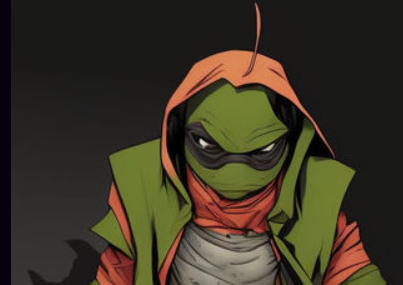
\includegraphics{Screenshot_2023-10-03_204548.png}
\caption{Screenshot 2023-10-03 204548.png}
\end{figure}

Informazioni Generali

Età:

Data di nascita:

Luogo di nascita:

Razza:

Classe:

Alleati:

Nemesi:

Alias:

Professione:

\begin{center}\rule{0.5\linewidth}{0.5pt}\end{center}

\subsection{1. Descrizione Generale}\label{descrizione-generale}

\begin{center}\rule{0.5\linewidth}{0.5pt}\end{center}

\begin{figure}
\centering
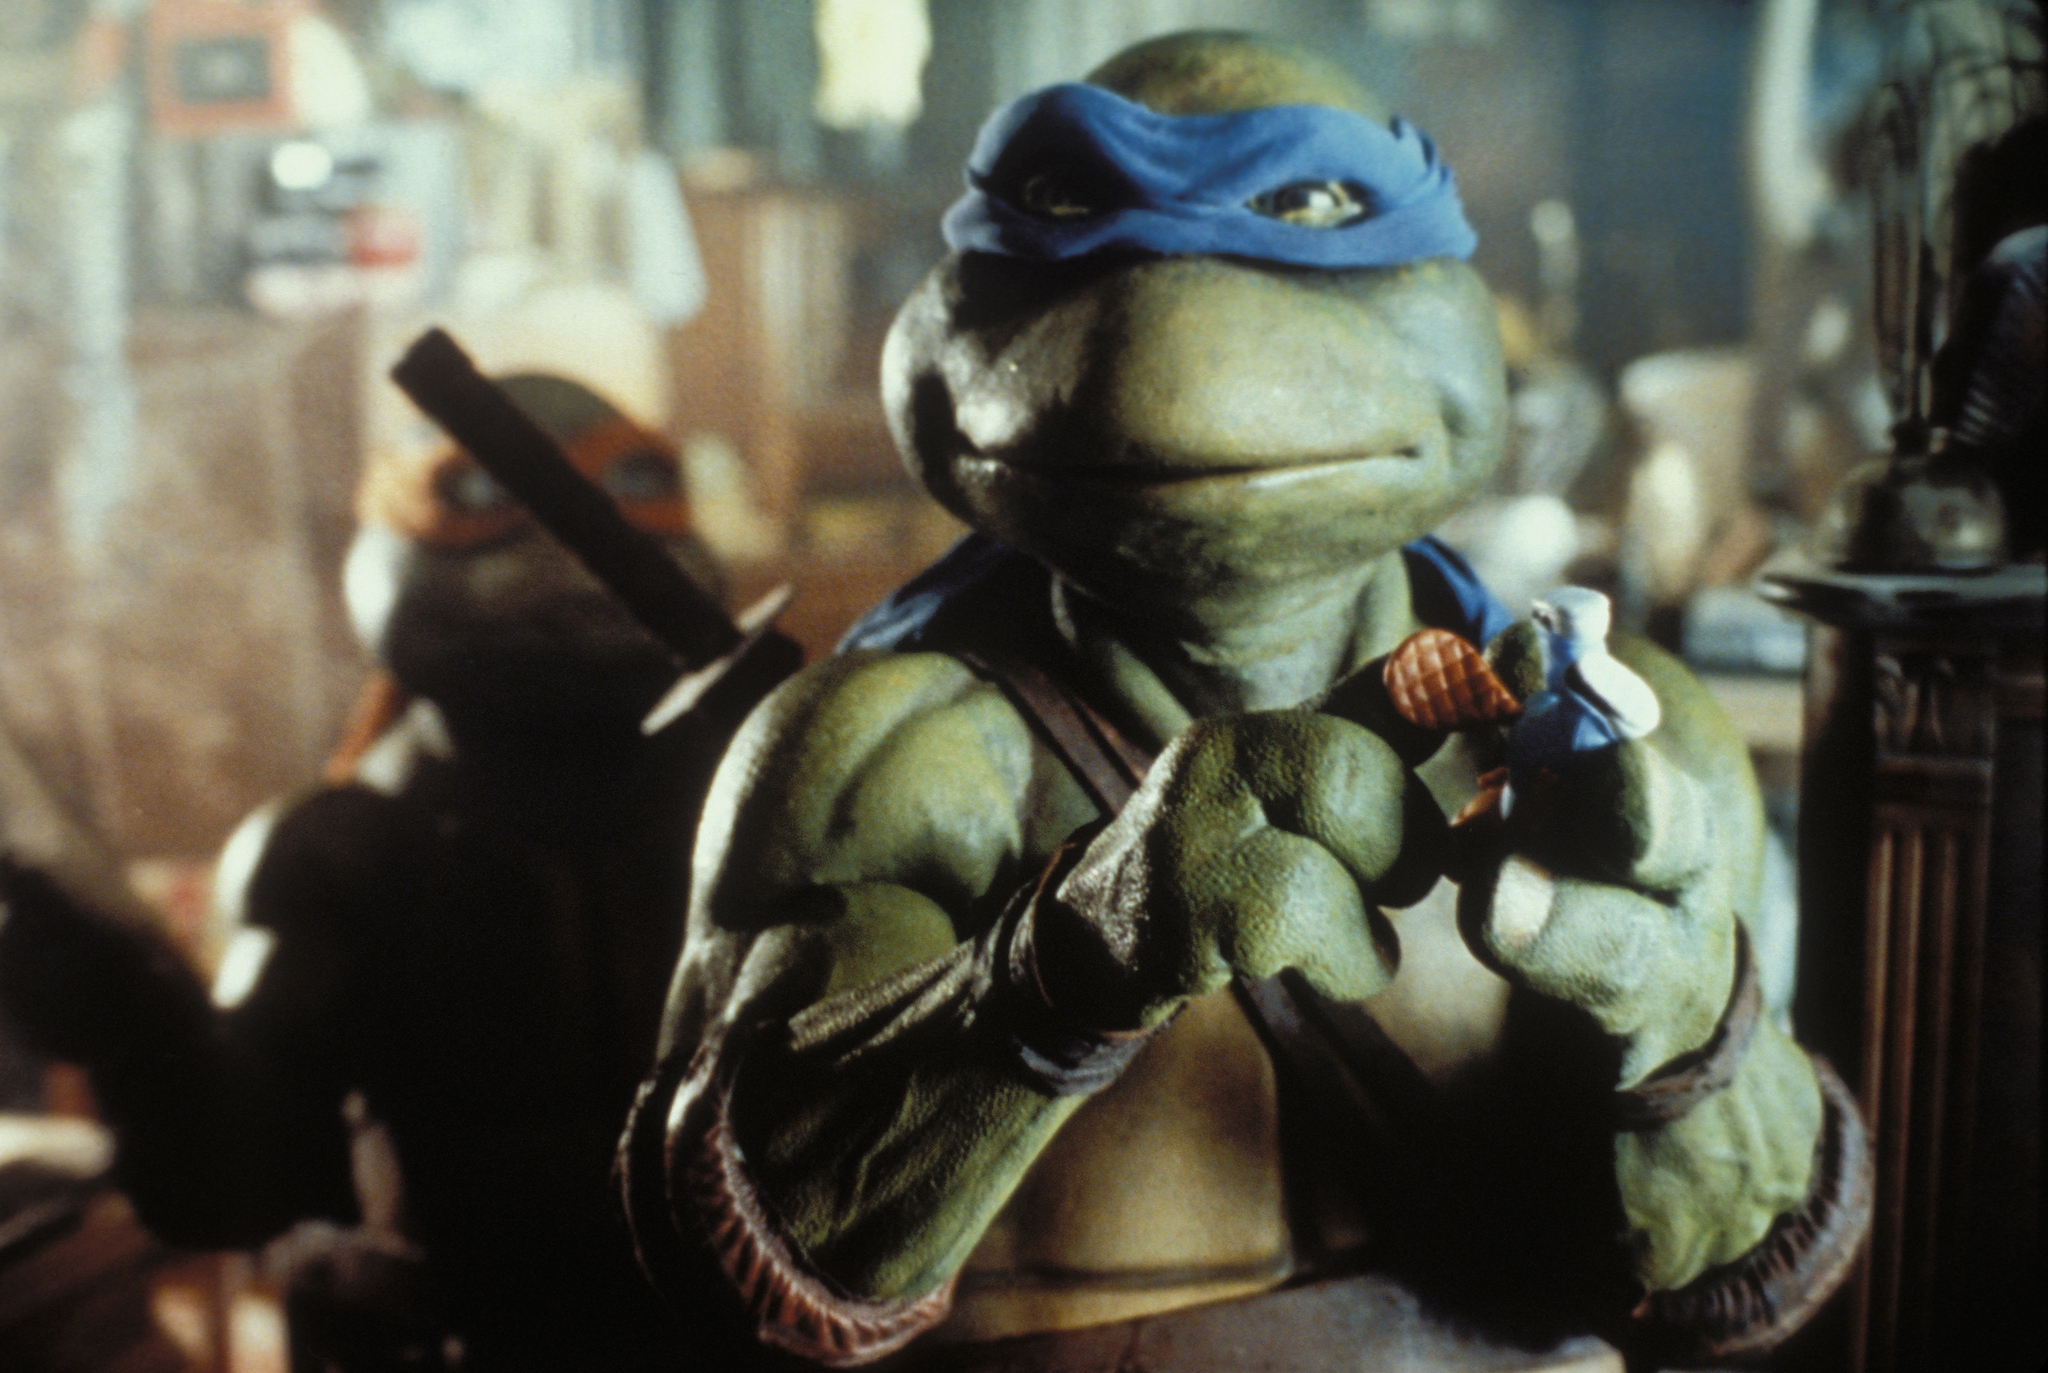
\includegraphics{foto_caravaggio.jpg}
\caption{foto caravaggio.jpg}
\end{figure}

Caravaggio è un monaco turtlefolk guerriero. La sua pelle verde scura e
il robusto guscio marrone lo distinguono tra gli altri della sua razza.
Caravaggio è noto per la sua lealtà, il suo coraggio e la sua
determinazione.

\begin{quote}
Citazione {[}location{]}
\end{quote}

\subsection{2. Biografia}\label{biografia}

\begin{center}\rule{0.5\linewidth}{0.5pt}\end{center}

Caravaggio è stato adottato da Splinter, un monaco mausefolk, insieme ai
suoi quattro fratelli. Splinter li ha cresciuti e addestrati alle arti
marziali, insegnando loro l'importanza della disciplina e della
protezione degli altri. Durante un viaggio in nave, un tremendo
naufragio ha separato Caravaggio dalla sua famiglia. Ha passato anni a
cercarla, senza mai darsi per vinto, ma non l'ha mai trovata.

\subsection{3. Carriera}\label{carriera}

\begin{center}\rule{0.5\linewidth}{0.5pt}\end{center}

Caravaggio ha trovato una nuova casa nelle terre di Valtara, dove ha
messo le sue abilità da combattente a servizio della gilda dei
Protettori. La sua esperienza in combattimento lo ha reso un membro
prezioso dell'organizzazione, impegnato a proteggere la regione dagli
innumerevoli pericoli che la minacciano. Il suo impegno nella gilda è
stato fonte di grande orgoglio, e ha dimostrato di essere un leader
calmo e risoluto quando è necessario.

\subsection{4. Personalità}\label{personalituxe0}

\begin{center}\rule{0.5\linewidth}{0.5pt}\end{center}

Caravaggio è noto per la sua lealtà e il suo coraggio. È determinato a
proteggere gli altri dopo aver perso la sua famiglia nel naufragio. Il
principale obiettivo di Caravaggio è riunirsi con i suoi fratelli e con
il suo mentore Splinter. Nel frattempo, si impegna a proteggere Valtara
e le persone che la abitano dai molteplici pericoli che la circondano.
La ricerca dei suoi fratelli è un impegno personale che lo guida in ogni
azione che intraprende.

\subsection{A. Coinvolgimenti in Eventi
Recenti}\label{a.-coinvolgimenti-in-eventi-recenti}

\begin{center}\rule{0.5\linewidth}{0.5pt}\end{center}

\href{Untitled\%20Database\%2001e713b9a2ea4437bbcda3f45f19839d.csv}{Untitled
Database}

\subsection{A. Scheda Personaggio}\label{a.-scheda-personaggio}

\begin{center}\rule{0.5\linewidth}{0.5pt}\end{center}

\href{Info\%20PG\%203043847ed767416a900f6caae343507f.csv}{Info PG}

\subsubsection{Statistiche e abilità}\label{statistiche-e-abilituxe0}

\begin{center}\rule{0.5\linewidth}{0.5pt}\end{center}

\href{Abilita\%CC\%80\%2088163116ffda4d90b9be228ef46e256c.csv}{Abilità}

\subsubsection{Lista magie}\label{lista-magie}

\subsection{B. Galleria Immagini}\label{b.-galleria-immagini}

\subsection{A. Descrizione Originale}\label{a.-descrizione-originale}

\begin{center}\rule{0.5\linewidth}{0.5pt}\end{center}
